\documentclass[border=12pt]{standalone}
\usepackage{tikz}
\usetikzlibrary{shapes.geometric, arrows.meta, positioning, calc, fit, backgrounds}
\usepackage{fontspec}
\setmainfont{DejaVu Sans}

\begin{document}
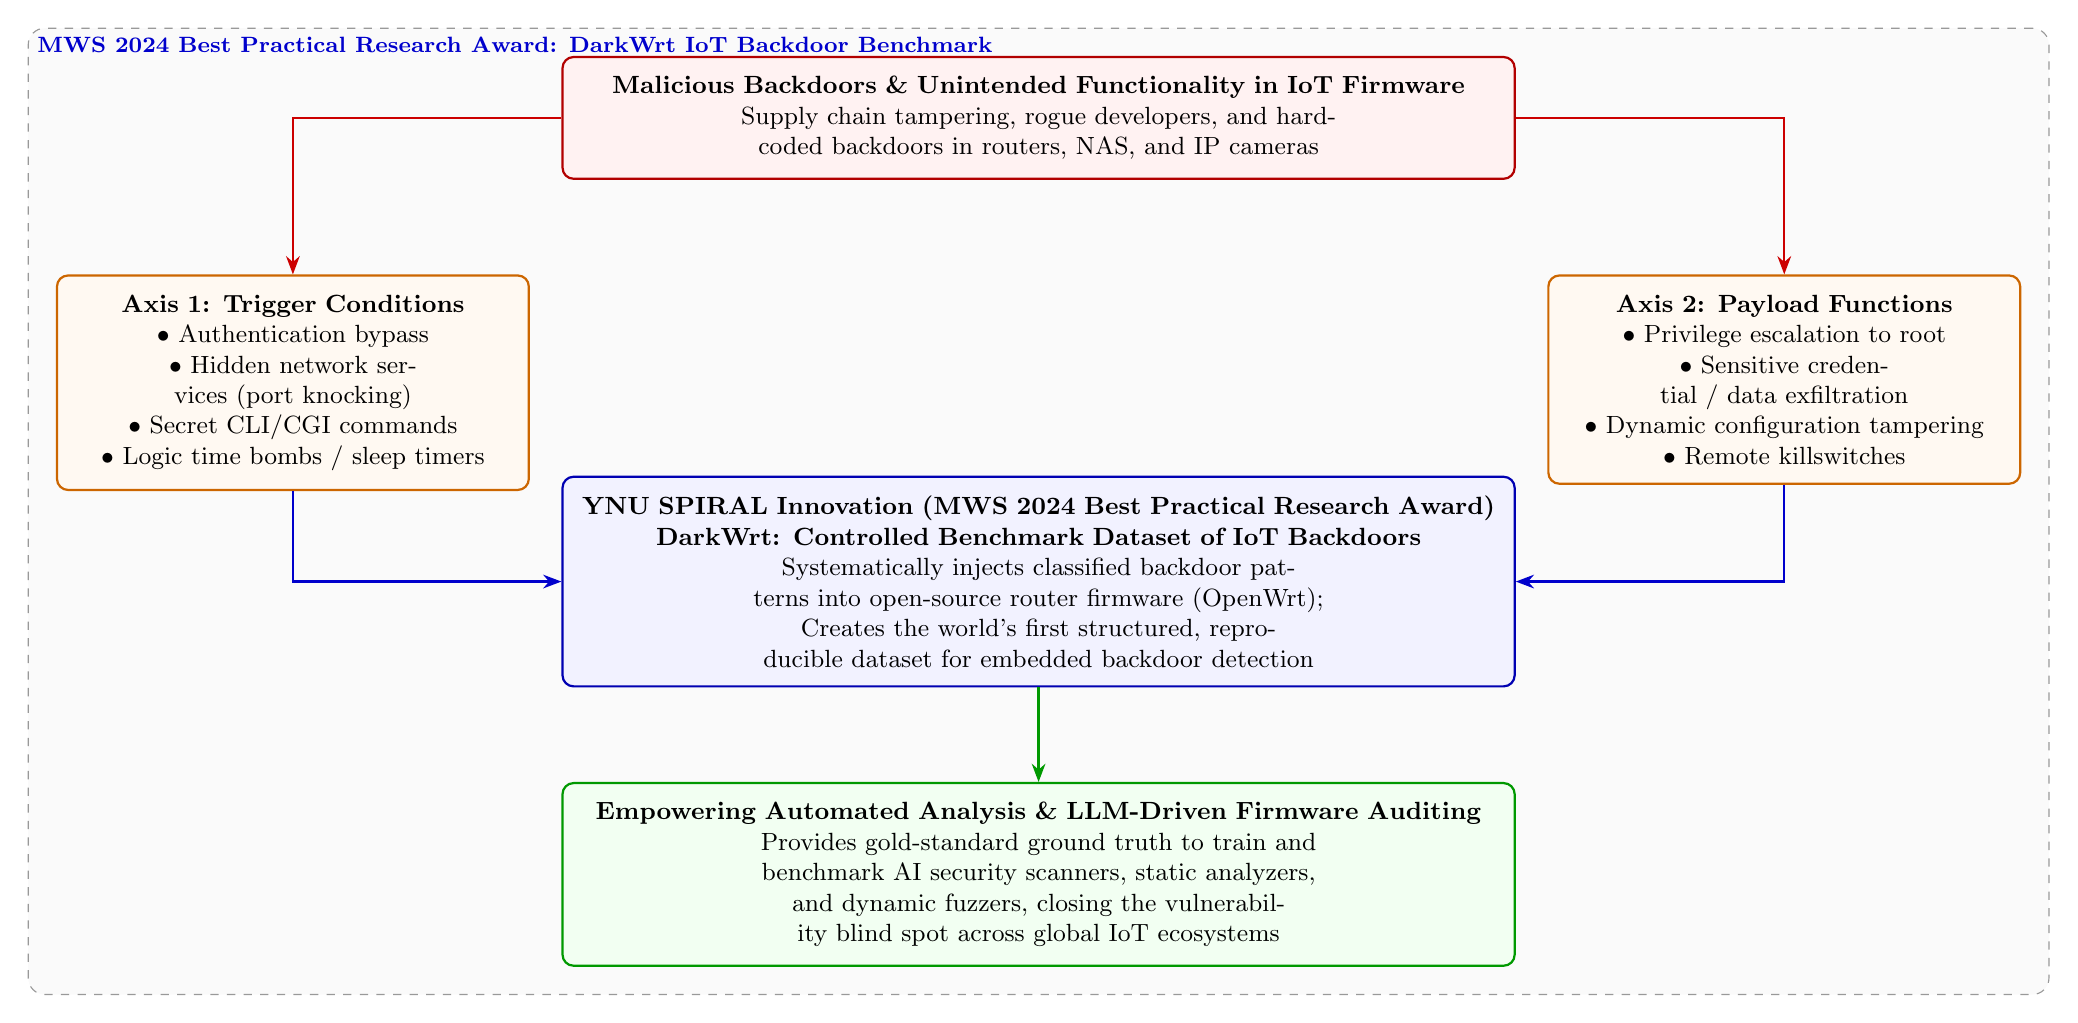
\begin{tikzpicture}[
    font=\small,
    >=Stealth,
    node distance=1.2cm,
    block/.style={rectangle, draw=blue!70!black, fill=blue!5, rounded corners=4pt, thick, align=center, inner sep=7pt},
    alertblock/.style={rectangle, draw=red!70!black, fill=red!5, rounded corners=4pt, thick, align=center, inner sep=7pt},
    greenblock/.style={rectangle, draw=green!60!black, fill=green!5, rounded corners=4pt, thick, align=center, inner sep=7pt},
    amberblock/.style={rectangle, draw=orange!80!black, fill=orange!5, rounded corners=4pt, thick, align=center, inner sep=7pt},
    groupbox/.style={draw=black!40, dashed, rounded corners=6pt, fill=black!2, inner sep=10pt}
]

    % Top: The Hidden Threat in IoT Firmware
    \node[alertblock, text width=11.6cm] (threat) {\textbf{Malicious Backdoors \& Unintended Functionality in IoT Firmware}\\Supply chain tampering, rogue developers, and hardcoded backdoors in routers, NAS, and IP cameras};

    % Left: Two-Axis Taxonomy
    \node[amberblock, below left=1.2cm and 0.4cm of threat, text width=5.5cm] (triggers) {\textbf{Axis 1: Trigger Conditions}\\$\bullet$ Authentication bypass\\$\bullet$ Hidden network services (port knocking)\\$\bullet$ Secret CLI/CGI commands\\$\bullet$ Logic time bombs / sleep timers};

    \node[amberblock, below right=1.2cm and 0.4cm of threat, text width=5.5cm] (functions) {\textbf{Axis 2: Payload Functions}\\$\bullet$ Privilege escalation to root\\$\bullet$ Sensitive credential / data exfiltration\\$\bullet$ Dynamic configuration tampering\\$\bullet$ Remote killswitches};

    \draw[->, thick, red!80!black] (threat) -| (triggers);
    \draw[->, thick, red!80!black] (threat) -| (functions);

    % Middle: Proposed Dataset: DarkWrt
    \node[block, below=1.2cm of $(triggers)!0.5!(functions)$, text width=11.6cm] (darkwrt) {\textbf{YNU SPIRAL Innovation (MWS 2024 Best Practical Research Award)}\\\textbf{DarkWrt: Controlled Benchmark Dataset of IoT Backdoors}\\Systematically injects classified backdoor patterns into open-source router firmware (OpenWrt);\\Creates the world's first structured, reproducible dataset for embedded backdoor detection};

    \draw[->, thick, blue!80!black] (triggers) |- (darkwrt);
    \draw[->, thick, blue!80!black] (functions) |- (darkwrt);

    % Bottom: Future Defense Impact
    \node[greenblock, below=1.2cm of darkwrt, text width=11.6cm] (impact) {\textbf{Empowering Automated Analysis \& LLM-Driven Firmware Auditing}\\Provides gold-standard ground truth to train and benchmark AI security scanners, static analyzers,\\and dynamic fuzzers, closing the vulnerability blind spot across global IoT ecosystems};

    \draw[->, thick, green!60!black] (darkwrt) -- (impact);

    \begin{scope}[on background layer]
        \node[groupbox, fit=(threat) (triggers) (functions) (darkwrt) (impact), label={[anchor=north west, font=\footnotesize\bfseries, blue!80!black]north west:MWS 2024 Best Practical Research Award: DarkWrt IoT Backdoor Benchmark}] {};
    \end{scope}

\end{tikzpicture}
\end{document}
